% !TeX root = ../RegT4.tex
% vim: ts=2 sw=2 spell:

\section{State Space Models}

\begin{figure}
	\centering
	\resizebox{\linewidth}{!}{
		\begin{tikzpicture}[very thick]
  \matrix[
    column sep = 6mm, row sep = 4mm,
  ]{
    &&& \node[rtbox] (D) {\(\mathbf{D}\)}; \\

    \node[rtsplit] (U) {};
      & \node[rtbox] (B) {\(\mathbf{B}\)};
      & \node[rtsum] (dX) {};
        \node[above = 0mm of dX] {\(\dot{\mathbf{x}}\)};
      & \node[rtint] (I) {};
      & \node[rtsplit] (X) {};
        \node[above = 0mm of X] {\(\mathbf{x}\)};
      & \node[rtbox] (C) {\(\mathbf{C}\)};
      & \node[rtsum] (Y) {}; \\[1mm]

    &&& \node[rtbox] (A) {\(\mathbf{A}\)}; \\
  };

  \draw[->]
    (U) -- ++(-1,0) node[left] {\(\mathbf{u}\)}
    (U) edge (B)
    (B) edge (dX)
    (dX) edge (I)
    (I) -- (X)
    (X) edge (C)
    (C) edge (Y)
    (Y) -- ++(1,0) node[right] {\(\mathbf{y}\)}
  ;

  \draw[->] (U) |- (D);
  \draw[->] (D) -| (Y);

  \draw[->] (X) |- (A);
  \draw[->] (A) -| (dX);

\end{tikzpicture}

	}
	\caption{
		State space model of a LTI system.
		\label{fig:ss-model}
	}
\end{figure}

\subsection{Introduction}

In modern control theory a \emph{state} of a dynamic system is the smallest set of variables (called \emph{state variables}) such that the knowledge of these variables at \(t = t_0\), together with the knowledge of the input for \(t \geq t_0\), completely determines the behavior of the system for any time \(t \geq t_0\).

\subsection{State Space Equations}

The state space equations are, in their most general form, a set of first order differential equations and a set of outputs:
\begin{align*}
	\dot{\vec{x}} &= \vec{f}(\vec{x}, \vec{u}, t) \\
	\vec{y} &= \vec{g}(\vec{x}, \vec{u}, t).
\end{align*}
This can describe any system because higher order differential equations can (practically) always be rewritten as a set of first order differential equations. In the case where the system is \emph{linear} they can be rewritten using linear algebra:
\begin{align*}
	\dot{\vec{x}}(t) & = \mx{A} \vec{x}(t) + \mx{B} \vec{u}(t), \\
	\vec{y}(t)       & = \mx{C} \vec{x}(t) + \mx{D} \vec{u}(t),
\end{align*}
where \(
	\mx{A} \in \mathbb{R}^{n \times n},
	\mx{B} \in \mathbb{R}^{n \times m},
	\mx{C} \in \mathbb{R}^{p \times n},
	\mx{D} \in \mathbb{R}^{p \times m}
\)
(see figure \ref{fig:ss-model}).  In general in a time varying system all four matrices are actually functions of time (\(\mx{A} = \mx{A}(t), \ldots\)). Whereas for \emph{linear time invariant} (LTI) systems they are constants.

\subsection{Linearization of non LTI systems}

In general dynamics are not LTI systems, however it is possible to create linear approximation of complex dynamics around a \emph{set point} \((\vec{x}_0, \vec{u}_0)\), if it is also a fixed point (that means \(\vec{f}(\vec{x}_0, \vec{u}_0) = \vec{0}\) and \(\vec{g}(\vec{x}_0, \vec{u}_0) = \vec{y}_0\)), by computing the four Jacobian matrices:
\begin{align*}
	\mx{A} &= \frac{\partial\vec{f}}{\partial\vec{x}} (\vec{x}_0, \vec{u}_0), &
	\mx{B} &= \frac{\partial\vec{f}}{\partial\vec{u}} (\vec{x}_0, \vec{u}_0), \\
	\mx{C} &= \frac{\partial\vec{g}}{\partial\vec{x}} (\vec{x}_0, \vec{u}_0), &
	\mx{D} &= \frac{\partial\vec{g}}{\partial\vec{u}} (\vec{x}_0, \vec{u}_0).
\end{align*}
Then the differences \(\Delta\vec{x} = \vec{x} - \vec{x}_0\), \(\Delta\vec{u} = \vec{u} - \vec{u}_0\) are used in the model:
\begin{align*}
	\Delta\dot{\vec{x}}(t) & = \mx{A} \Delta\vec{x} + \mx{B} \Delta\vec{u}, \\
	\Delta\vec{y}(t)       & = \mx{C} \Delta\vec{x} + \mx{D} \Delta\vec{u}.
\end{align*}

\subsection{Time-Domain Solutions}

\subsubsection{Homogeneous Case}

To solve for the solution of the system at rest (no inputs)
\[
	\dot{\vec{x}} = \mx{A} \vec{x},
\]
we assume that the solution is a power series in \(t\), or
\[
	\vec{x}(t) = \vec{b}_0 + \vec{b}_1 t + \vec{b}_2 t^2 + \dots + \vec{b}_k t^k + \dots.
\]
Substituting into the differential equation yields a solution
\[
	\vec{x}(t) = \underbrace{\left(
		\mx{I} + \mx{A} t + \frac{1}{2!} \mx{A}^2 t^2 + \dots
		+ \frac{1}{k!} \mx{A}^k t^k + \dots
	\right)}_{\text{Matrix exponential } e^{\mx{A}t}} \vec{x}(0),
\]
which looks like the power series for the exponential function. Thus we define it to be the \emph{matrix exponential} and write the solution as
\[
	\vec{x}(t) = e^{\mx{A}t} \vec{x}(0).
\]
The matrix exponential has the property that
\[
	e^{\mx{A}(t + s)} = e^{\mx{A}t} e^{\mx{A}s},
\]
and in particular when \(s = -t\) then the expression equals the identity matrix. Thus the inverse of \(e^{\mx{A}t}\) is \(e^{-\mx{A}t}\) and always exists. It is important to note that
\[
	e^{(\mx{A} + \mx{B}) t} \neq e^{\mx{A}t} e^{\mx{B}t},
\]
unless we are in the very special case when \(\mx{A}\mx{B} = \mx{B}\mx{A}\).

\subsubsection{Transition Matrix}

The result of the exponential matrix is of such relevance that it has a special name. The expression
\[
	\mx{\Phi}(t) = e^{\mx{A} t}
\]
is called the \emph{transition matrix}, since it describes how the initial conditions change. The transition matrix has some important algebraic properties which are listed below:
\begin{gather*}
	\mx{\Phi}(0)
		= e^{\mx{A} 0}
		= \mx{I}, \\
	\mx{\Phi}^{-1}(t)
		= \left(e^{\mx{A}t}\right)^{-1}
		= \mx{\Phi}(-t), \\
	\mx{\Phi}(t)^{n}
		= \left(e^{\mx{A}t}\right)^{n}
		= \mx{\Phi}(nt), \\
	\mx{\Phi}(t_1 + t_2)
		= e^{\mx{A}(t_1 + t_2)}
		= \mx{\Phi}(t_1) \mx{\Phi}(t_2)
		= \mx{\Phi}(t_2) \mx{\Phi}(t_1), \\
	\mx{\Phi}(t_2 - t_1) \mx{\Phi}(t_1 - t_0)
		= \mx{\Phi}(t_2 - t_0)
		% = \mx{\Phi}(t_1 - t_0) \mx{\Phi}(t_2 - t_1)
		\\
	\dot{\mx{\Phi}}(t) = \mx{A}\mx{\Phi}(t)
	.
\end{gather*}
A noteworthy result from the last property is that
\[
	\mx{A} = \dot{\mx{\Phi}}(t) \mx{\Phi}^{-1}(t)
	= \dot{\mx{\Phi}}(t) \mx{\Phi}(-t).
\]
Finally, in the case when \(\mx{A}\) is a diagonal matrix with entries \(\lambda_1, \ldots, \lambda_n\) then
\[
	\mx{\Phi}(t) = e^{\mx{A} t} = \begin{bmatrix}
		e^{\lambda_1 t} & & 0 \\
		& \ddots \\
		0 & & e^{\lambda_n t}
	\end{bmatrix}.
\]

\begin{figure}
	\centering
	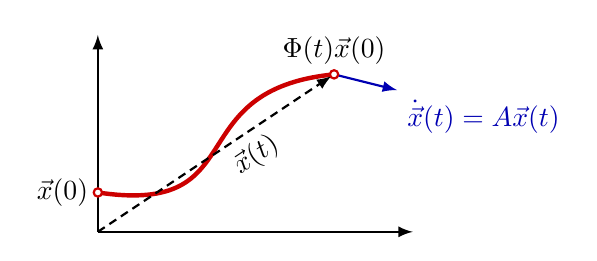
\begin{tikzpicture}[
			dot/.style = {
				circle, thick,
				draw = red!80!black, fill = white,
				minimum size = 3pt, inner sep = 0pt,
			}
		]
		\draw[thick, -latex] (0, 0) -- (4, 0);
		\draw[thick, -latex] (0, 0) -- (0, 2.5);

		\draw[ultra thick, red!80!black]
			(0, .5) coordinate (S) .. controls (2, .2) and (1, 1.8) .. (3, 2)
			node[outer sep = 0, inner sep = 1pt] (E) {};

		\draw[thick, black, densely dashed, -latex]
			(0, 0) -- (E) node[midway, sloped, below right] {\(\vec{x}(t)\)};

		\draw[thick, blue!70!black, -latex]
			(E) -- ++(.8, -.2) node[below right] {\(\dot{\vec{x}}(t) = \mx{A} \vec{x}(t)\)};

		\node[left] at (S) {\(\vec{x}(0)\)};
		\node[above] at (E) {\(\mx{\Phi}(t) \vec{x}(0)\)};

		\node[dot] at (S) {};
		\node[dot] at (E) {};
	\end{tikzpicture}
	\caption{
		Interpretation of the \(\mx{A}\) and \(\mx{\Phi}\) matrices.
		\label{fig:ss-matrix-interp}
	}
\end{figure}

\subsubsection{Nonhomogeneous Case} \label{sec:ss-sol-time-nonh}

To expand the previous result, in the more general case when
\[
	\dot{\vec{x}} = \mx{A} \vec{x} + \mx{B} \vec{u},
\]
a few steps that are the same as in the scalar case give the solution
\[
	\vec{x}(t) = e^{\mx{A} t} \vec{x}(0)
		+ \int_0^t e^{\mx{A} (t - \tau)} \mx{B} \vec{u}(\tau) d\tau,
\]
which can also be written using the transition matrix as:
\[
	\vec{x}(t) = \mx{\Phi}(t) \vec{x}(0)
		+ \int_0^t \mx{\Phi}(t - \tau) \mx{B} \vec{u}(\tau) d\tau.
\]

\subsection{Laplace \(s\)-Domain Solution}

\subsubsection{Transfer Matrix}

By taking the Laplace transform the state space equations of an LTI system they become:
\begin{align*}
	s\vec{X}(s) - \vec{x}(0) & = \mx{A} \vec{X}(s) + \mx{B} \vec{U}(s), \\
	\vec{Y}(s)              & = \mx{C} \vec{X}(s) + \mx{D} \vec{U}(s).
\end{align*}
Similarly to the one dimensional case it is now possible to define the more general equivalent of a transfer function:
\[
	\mx{G}(s) = \mx{C}\left(s\mx{I} - \mx{A}\right)^{-1} \mx{B} + \mx{D},
\]
which is the \emph{transfer matrix}.

\subsubsection{Impulse Response}

The inverse Laplace transform of the transfer matrix is the \emph{impulse response}. However, setting \(\vec{u}(t) = \vec{\delta}(t)\) will also give the impulse response. By taking the result in section \ref{sec:ss-sol-time-nonh} and substituting into the output equation, we get that with a Dirac delta as input
\[
	\vec{g}(t) = \mx{C} \mx{\Phi}(t) \mx{B} + \mx{D} \vec{\delta}(t).
\]

\subsection{Controllability}

A system is said to be \emph{controllable} at time \(t_0\) if it is possible my means of an unconstrained control vector to transfer the system from any initial state \(\vec{x}(t_0)\) to any other state in a finite interval of time. To check if a system is completely controllable there is the \(n\times  nm\) \emph{controllability matrix}
\[
	\mx{Q}_c = \begin{bmatrix}
		\mx{B} & \mx{A}\mx{B} & \cdots & \mx{A}^{n-1}\mx{B}
	\end{bmatrix}.
\]
If \(\rank \mx{Q}_c < n\) (has less than \(n\) linearly independent rows), or in the case when \(\mx{Q}_c\) is a square matrix \(\det \mx{Q}_c = 0\), then the system is not totally state controllable.

It is also possible to determine the controllability from the transfer function (or matrix) of a system. It can be shown that if cancellation occurs (German: \textsl{Polkürzung}), then the system cannot be controlled in the direction of the canceled mode.

\subsection{Observability}

In the same (too) abstract spirit as in the controllability: a system is said to be \emph{observable} at time \(t_0\) if, with the system in state \(\vec{x}(t_0)\), it is possible to determine this state from the observation of the output over a finite time interval. The observability can be determined through the \(np \times n\) \emph{observability matrix}
\[
	\mx{Q}_o = \begin{bmatrix}
		\mx{C} \\ \mx{C}\mx{A} \\ \vdots \\ \mx{C}\mx{A}^{n-1}
	\end{bmatrix} = \begin{bmatrix}
		\mx{C}^* & \mx{A}^* \mx{C}^* & \cdots & (\mx{A}^*)^{n-1}\mx{C}^*
	\end{bmatrix},
\]
where the asterisk is the conjugate transpose (for real matrices \(\mx{A}^* = \mx{A}^\mathsf{T}\)). The system is observable only if \(\rank \mx{Q} \geq n\) (there are at least \(n\) linearly independent rows).

In terms of the transfer function: if cancellation occurs in the transfer function then the canceled mode cannot be observed for the output. In other words, no cancellation is a necessary and sufficient condition for total observability.

\subsection{Stability} \label{sec:stability}

A state space model system is stable is the \(\mx{A}\) matrix is positive definite, which means that the real part of all eigenvalues \(\Re{\lambda_i} > 0\). Another way to determine if \(\mx{A}\) is positive definite is to test whether the quadratic expression \(\vec{x}^* \mx{A} \vec{x} > 0\) for all \(\vec{x} \neq \vec{0}\).

\subsection{Equivalent Representations}

In this section we assume without loss of generality that the system has a transfer function
\[
	\frac{Y(s)}{U(s)} = d + \frac{
		b_{n-1} s^{n-1} + b_{n-2} s^{n-2} + \cdots + b_1 s + b_0
	}{
		s^n + a_{n-1} s^{n-1} + \cdots + a_1 s + a_0
	}.
\]

\subsubsection{Controllable Canonical Form}

This form (German: \textsl{Regelungsnormalform}) is important in discussing the pole-placement approach. It is given by

% ugly trick, do not replicate
\par\vspace{.5em}\noindent\resizebox{\linewidth}{!}{
	\(\displaystyle
		\begin{bmatrix}
			\dot{x}_1 \\ \dot{x}_2 \\ \vdots \\ \dot{x}_{n-1} \\ \dot{x}_n
		\end{bmatrix}
		=
		\begin{bmatrix}
			0 & 1 & 0 & \dots & 0 \\
			0 & 0 & 1 & \dots & 0 \\
			\vdots & \vdots & \vdots & \ddots & \vdots \\
			0 & 0 & 0 & \dots & 1 \\
			-a_0 & -a_1 & -a_2 & \dots & -a_{n-1}
		\end{bmatrix}
		\begin{bmatrix}
			x_1 \\ x_2 \\ \vdots \\ x_{n-1} \\ x_n
		\end{bmatrix}
		+
		\begin{bmatrix}
			0 \\ 0 \\ \vdots \\ 0 \\ 1
		\end{bmatrix} u.
	\)
}
And the output is
\[
	y =
	\begin{bmatrix}
		b_0 & \dots & b_{n-1}
	\end{bmatrix}
	\vec{x}
	+ d u
	.
\]

\subsubsection{Observable Canonical Form}

This mode is similar to previous form, in fact, the \(\mx{A}\) matrix is the transposed version of the controllable form:

% ugly trick, do not replicate
\par\vspace{.5em}\noindent\resizebox{\linewidth}{!}{
	\(\displaystyle
		\begin{bmatrix}
			\dot{x}_1 \\ \dot{x}_2 \\ \vdots \\ \dot{x}_{n-1} \\ \dot{x}_n
		\end{bmatrix}
		=
		\begin{bmatrix}
			0 & 0 & 0 & \dots & -a_n \\
			1 & 0 & 0 & \dots & -a_{n-1} \\
			\vdots & \vdots & \vdots & \ddots & \vdots \\
			0 & 1 & 0 & \dots & -a_2 \\
			0 & 0 & 0 & \dots & -a_1
		\end{bmatrix}
		\begin{bmatrix}
			x_1 \\ x_2 \\ \vdots \\ x_{n-1} \\ x_n
		\end{bmatrix}
		+
		\begin{bmatrix}
			b_0 \\ b_1 \\ \vdots \\ b_{n-2} \\ b_{n-1}
		\end{bmatrix} u.
	\)
}

\subsubsection{Diagonal Form (Decoupling)}

An important form is when the \(\mx{A}\) matrix is diagonalized, i.e.
\[
	\begin{bmatrix}
		\dot{x}_1 \\ \dot{x}_2 \\ \vdots \\ \dot{x}_{n-1} \\ \dot{x}_n
	\end{bmatrix}
	=
	\begin{bmatrix}
		\lambda_1 \\
		& \lambda_2 \\
		& & \ddots \\
		& & & \lambda_{n-1} \\
		& & & & \lambda_n
	\end{bmatrix}
	\begin{bmatrix}
		x_1 \\ x_2 \\ \vdots \\ x_{n-1} \\ x_n
	\end{bmatrix}
	+
	\tilde{\mx{B}}\b{u}.
\]
In this representation the state variables are the \emph{eigenstates} of the system, and they are decoupled from each other. Since the diagonal contains the eigenvalues, as noted in the stability section \ref{sec:stability}, they describe the poles of the transfer function \(G(s)\), and therefore the stability of the system. In other words
\[
	\frac{Y(s)}{U(s)} =
	\frac{b_1 c_1}{s - \lambda_1} +
	\frac{b_2 c_2}{s - \lambda_2} + \dots +
	\frac{b_n c_n}{s - \lambda_{n-1}}.
\]

\subsubsection{Normal Jordan Form}

\todo{From Ogata.}

\subsection{Similarity Transform}

In the previous section there were many representation that are practical to use, but in fact there is nothing special about them. In fact, the state space can be transformed into an infinite number of other equivalent representations.

Given an arbitrary regular matrix \(\mx{P}\), the state space in \(\vec{x}\) can be brought into a new set of state variables \(\vec{x}' := \mx{P} \vec{x}\) by appropriately transforming the matrices as follows:
\begin{align*}
	\mx{A}' &:= \mx{P} \mx{A} \mx{P}^{-1}, &
	\mx{B}'	&:= \mx{P} \mx{B}, \\
	\mx{C}' &:= \mx{C} \mx{P}^{-1}, &
	\mx{D}' &:= \mx{D}.
\end{align*}

\subsection{Subsystem Aggregation}

\subsubsection{Series}

When after a subsystem 1 a subsystem 2 is connected in series the model of the entire path is
\begin{align*}
	\begin{bmatrix}
		\dot{\vec{x}}_1 \\ \dot{\vec{x}}_2
	\end{bmatrix}
	&=
	\begin{bmatrix}
			\mx{A}_1 & \mx{0} \\
			\mx{B}_2 \mx{C}_1 & \mx{A}_2 
	\end{bmatrix}
	\begin{bmatrix}
		\vec{x}_1 \\ \vec{x}_2
	\end{bmatrix}
	+
	\begin{bmatrix}
		\mx{B}_1 \\ \mx{B}_2 \mx{D}_1
	\end{bmatrix}
	\vec{u},
	\\
	\vec{y}
	&=
	\begin{bmatrix}
		\mx{D}_2 \mx{C}_1 & \mx{C}_2
	\end{bmatrix}
	\begin{bmatrix}
		\vec{x}_1 \\ \vec{x}_2
	\end{bmatrix}
	+
	\mx{D}_2 \mx{D}_1 \vec{u}.
\end{align*}

\subsubsection{Parallel}

When a subsystem 1 and a subsystem 2 are connected in parallel, the model of the entire system is
\begin{align*}
	\begin{bmatrix}
		\dot{\vec{x}}_1 \\ \dot{\vec{x}}_2
	\end{bmatrix}
	&=
	\begin{bmatrix}
			\mx{A}_1 & \mx{0} \\
			\mx{0} & \mx{A}_2 
	\end{bmatrix}
	\begin{bmatrix}
		\vec{x}_1 \\ \vec{x}_2
	\end{bmatrix}
	+
	\begin{bmatrix}
		\mx{B}_1 \\ \mx{B}_2
	\end{bmatrix}
	\vec{u},
	\\
	\vec{y}
	&=
	\begin{bmatrix}
		\mx{C}_1 & \mx{C}_2
	\end{bmatrix}
	\begin{bmatrix}
		\vec{x}_1 \\ \vec{x}_2
	\end{bmatrix}
	+
	(\mx{D}_2 + \mx{D}_1) \vec{u}.
\end{align*}

\subsubsection{Feedback}

When to a subsystem 1 a subsystem 2 is connected in the negative feedback path, the matrices of the entire system are
\begin{align*}
	\mx{A}' &:=
	\begin{bmatrix}
		\mx{A}_1 - \mx{B}_1 \mx{K}_1 \mx{D}_2 \mx{C}_1 &
		-\mx{B}_1 \mx{K}_1 \mx{C}_2 \\
		\mx{B}_2 \mx{K}_2 \mx{C}_1 &
		\mx{A}_2 - \mx{B}_2 \mx{K}_2 \mx{D}_1 \mx{C}_2
	\end{bmatrix},
	\\
	\mx{B}' &:= 
	\begin{bmatrix}
		\mx{B}_1 \mx{K}_1 \\ \mx{B}_2 \mx{K}_2 \mx{D}_1
	\end{bmatrix},
	\\
	\mx{C}' &:= 
	\begin{bmatrix}
		\mx{K}_2 \mx{C}_1 &
		-\mx{K} \mx{D}_1 \mx{C}_2
	\end{bmatrix}
	\\
	\mx{D}' &:= \mx{K}_2 \mx{D}_1,
\end{align*}
where \(\mx{K}_1 = (\mx{I} - \mx{D}_2 \mx{D}_1)^{-1}\) and  \(\mx{K}_2 = (\mx{I} - \mx{D}_1 \mx{D}_2)^{-1}\). In the case of a positive feedback the minus signs become pluses.

\subsection{Create a State Space Model from a Transfer Function}

\todo{Ogata and skript p. 169, also from a diagram on p. 171.}
